\documentclass[10pt, a4paper]{article}
\usepackage[margin=1in]{geometry}
\usepackage[colorlinks=true]{hyperref}
\usepackage{graphicx}
\renewcommand{\familydefault}{\sfdefault}
\usepackage{fontspec}
\setsansfont{DejaVu Sans}

\setlength{\parindent}{0pt}
\setlength{\parskip}{1cm}


\title{How to translate a book using Transifex}
\author{Siyavula Education}
\date{}



\begin{document}
\maketitle

\section*{What is Transifex?}

Transifex is an open-source computer aided translation tool. It is a web application that allows teams of people to manage and perform translations of texts. You can read more about Transifex here: \url{https://www.Transifex.com/}. Siyavula  runs its own copy of Transifex at  \url{http://translate.siyavula.com}, this is where you will do your translations.


\section*{Step 1: Registering a new user account}

Go to \url{http://translate.siyavula.com} in your browser. You should see something like:

\begin{center}
    \centerline{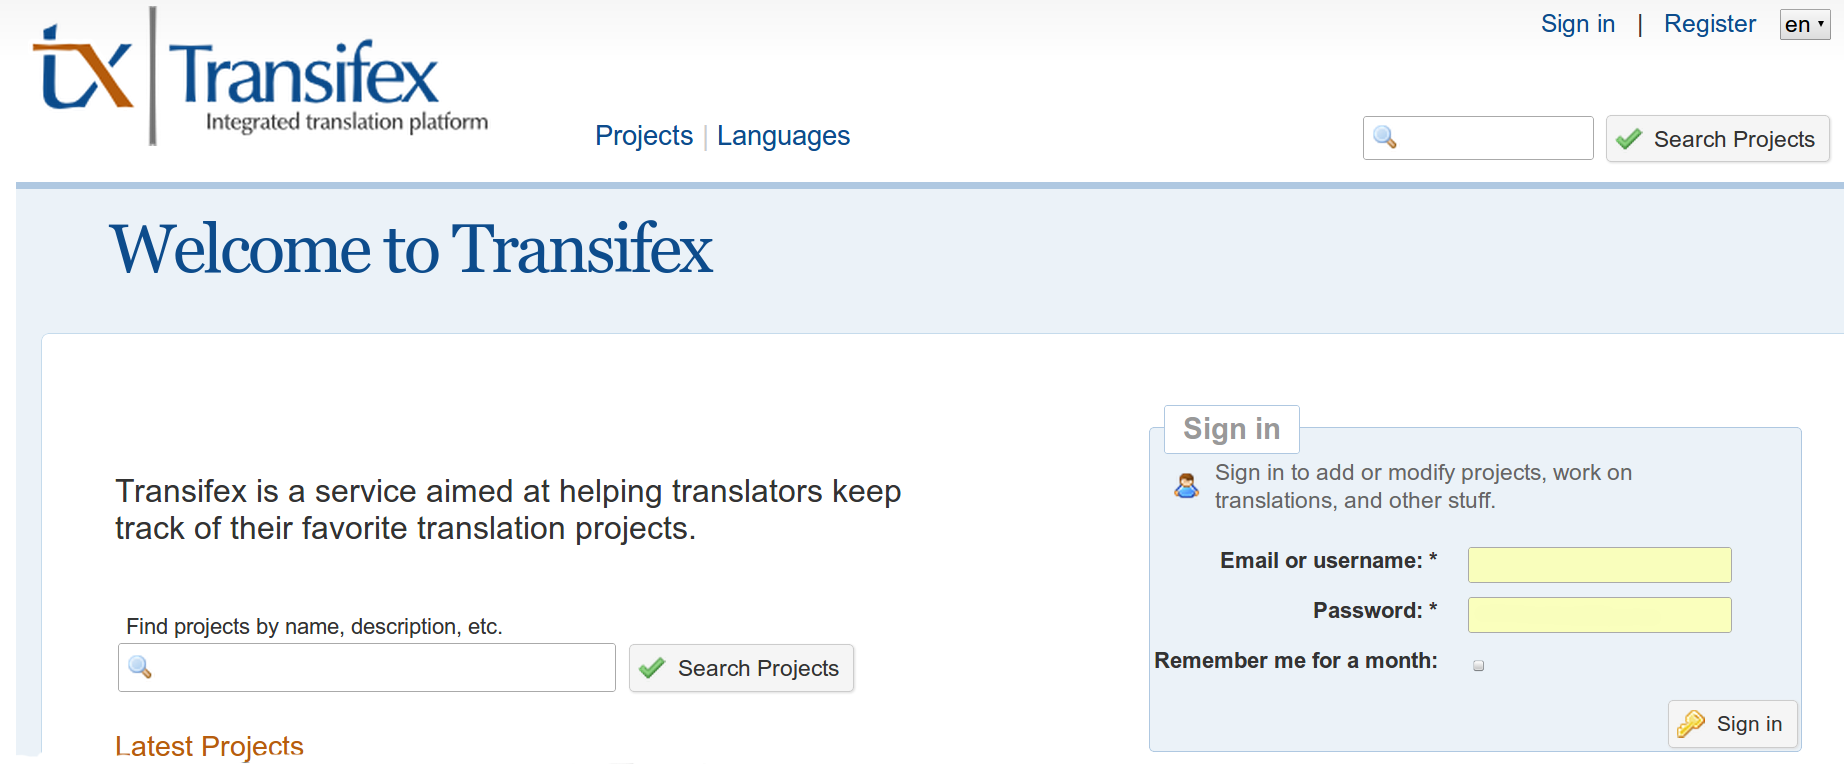
\includegraphics[width=0.8\paperwidth]{images/Screenshot.png}}
\end{center}
Click on the ``Register'' button in the top right corner to create a new account, if you have not done this already.


You will be taken to the registration page which looks like this:
\begin{center}
    \centerline{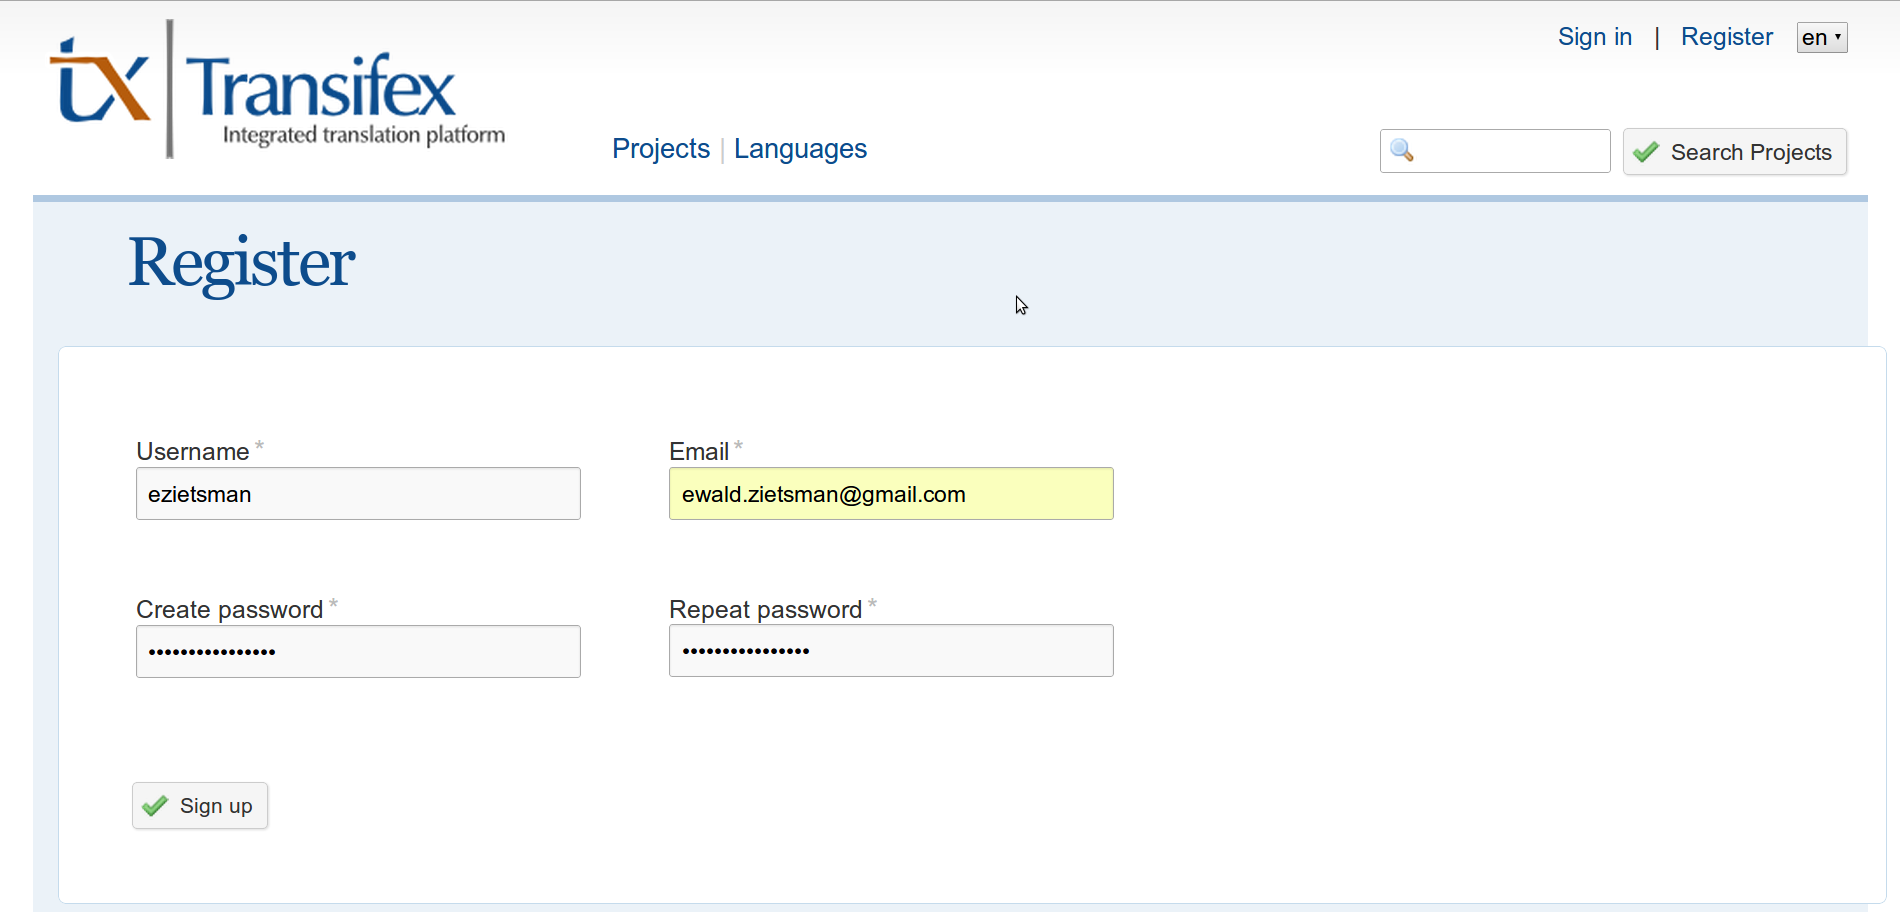
\includegraphics[width=0.8\paperwidth]{images/enterdetails.png}}
\end{center}
Please choose a username and enter a valid email address. Choose password and enter it into the two password boxes. Click in the ``Sign up'' button when you are done. You will receive an email at the address you entered. The email contains a link which you must click on to activate your account. You will then be taken to this page:
\begin{center}
    \centerline{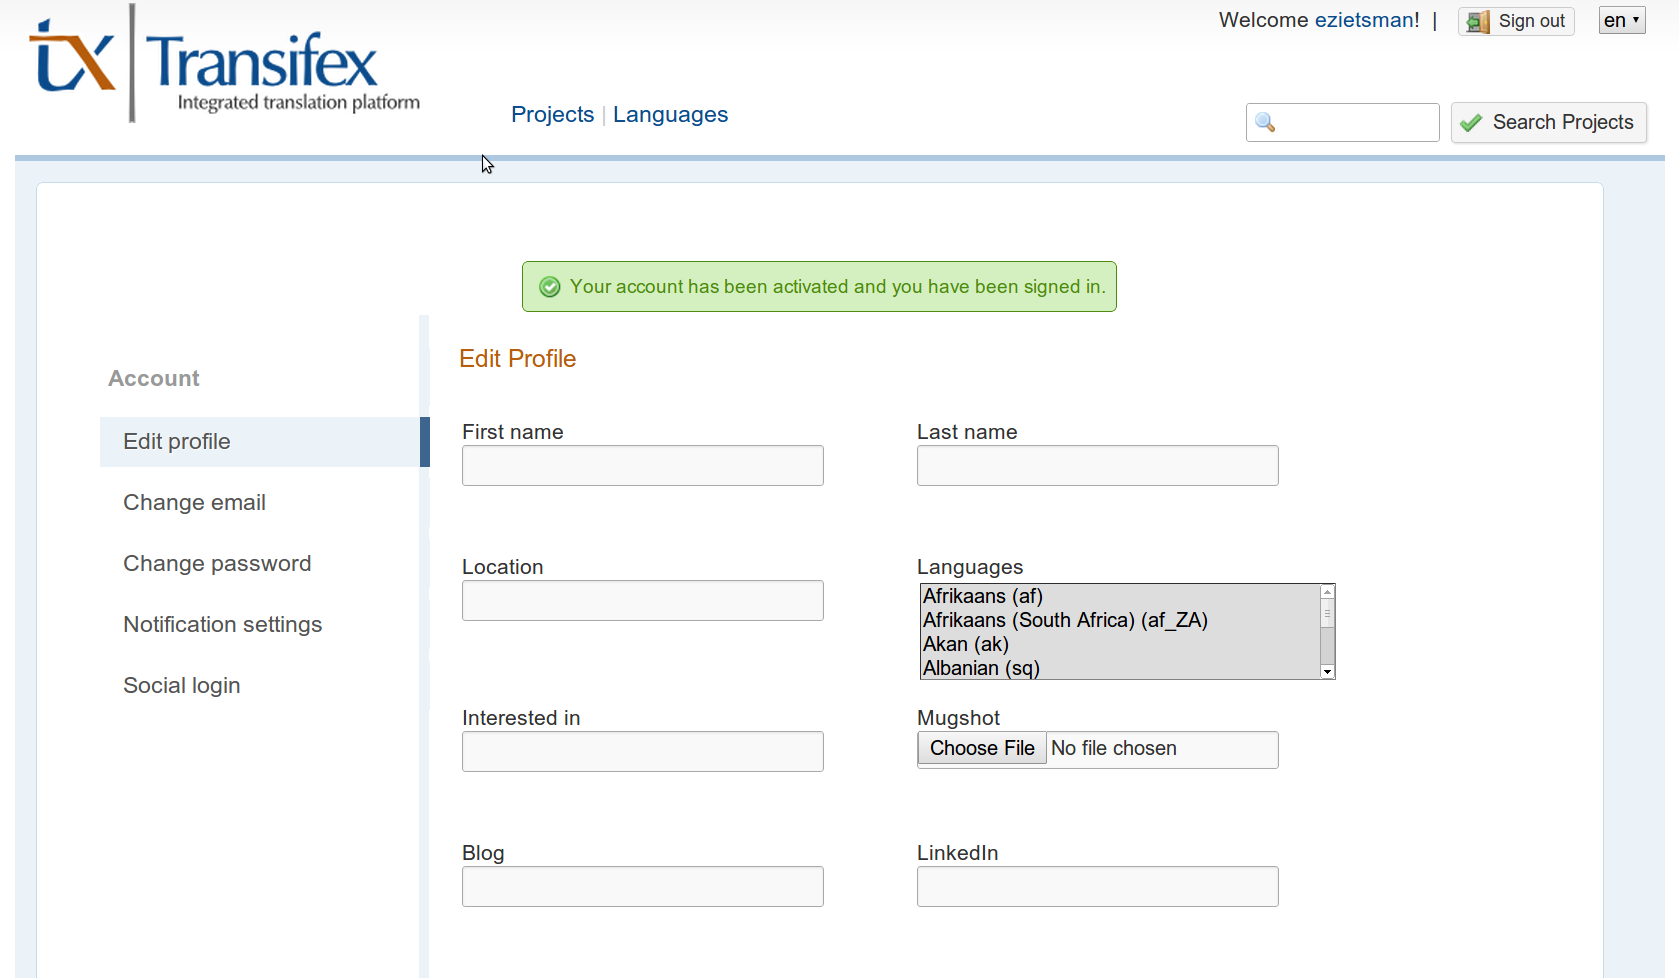
\includegraphics[width=0.8\paperwidth]{images/signedin.png}}
\end{center}



\section*{Step 2: Finding the project you will work on}

Let's assume you have been assigned to the ``Atomic Combinations 1'' resource under the ``Physical Sciences Grade 11'' project. Clicking on the ``Projects'' link at the top of the page should take you to a page that looks like this:
\begin{center}
    \centerline{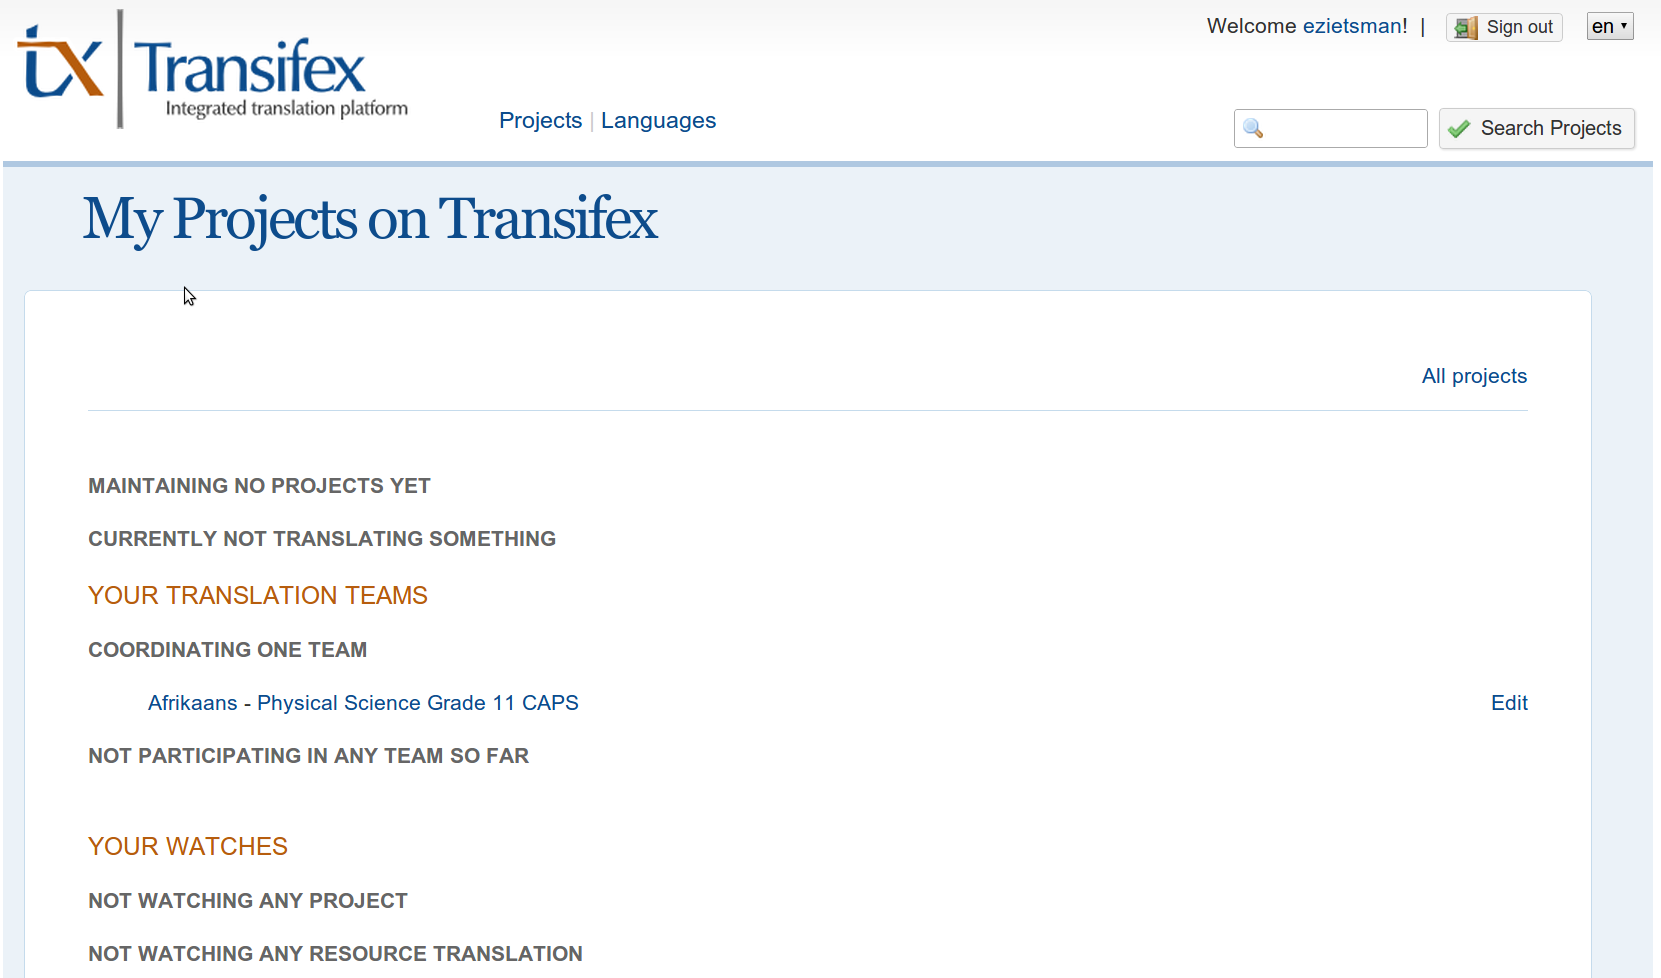
\includegraphics[width=0.8\paperwidth]{images/selectproject.png}}
\end{center}
If you are a member of any translation teams, you will see a link under ``Participating in xxx teams'' in the above image. Click on the link that says ``Physical Sciences Grade 11'' (or whichever project you are contributing to).

You will then see the resources that have been uploaded to the project. The Siyavula team will do this. Look for the link that says ``Atomic Combinations 1'' and click on it:
\begin{center}
    \centerline{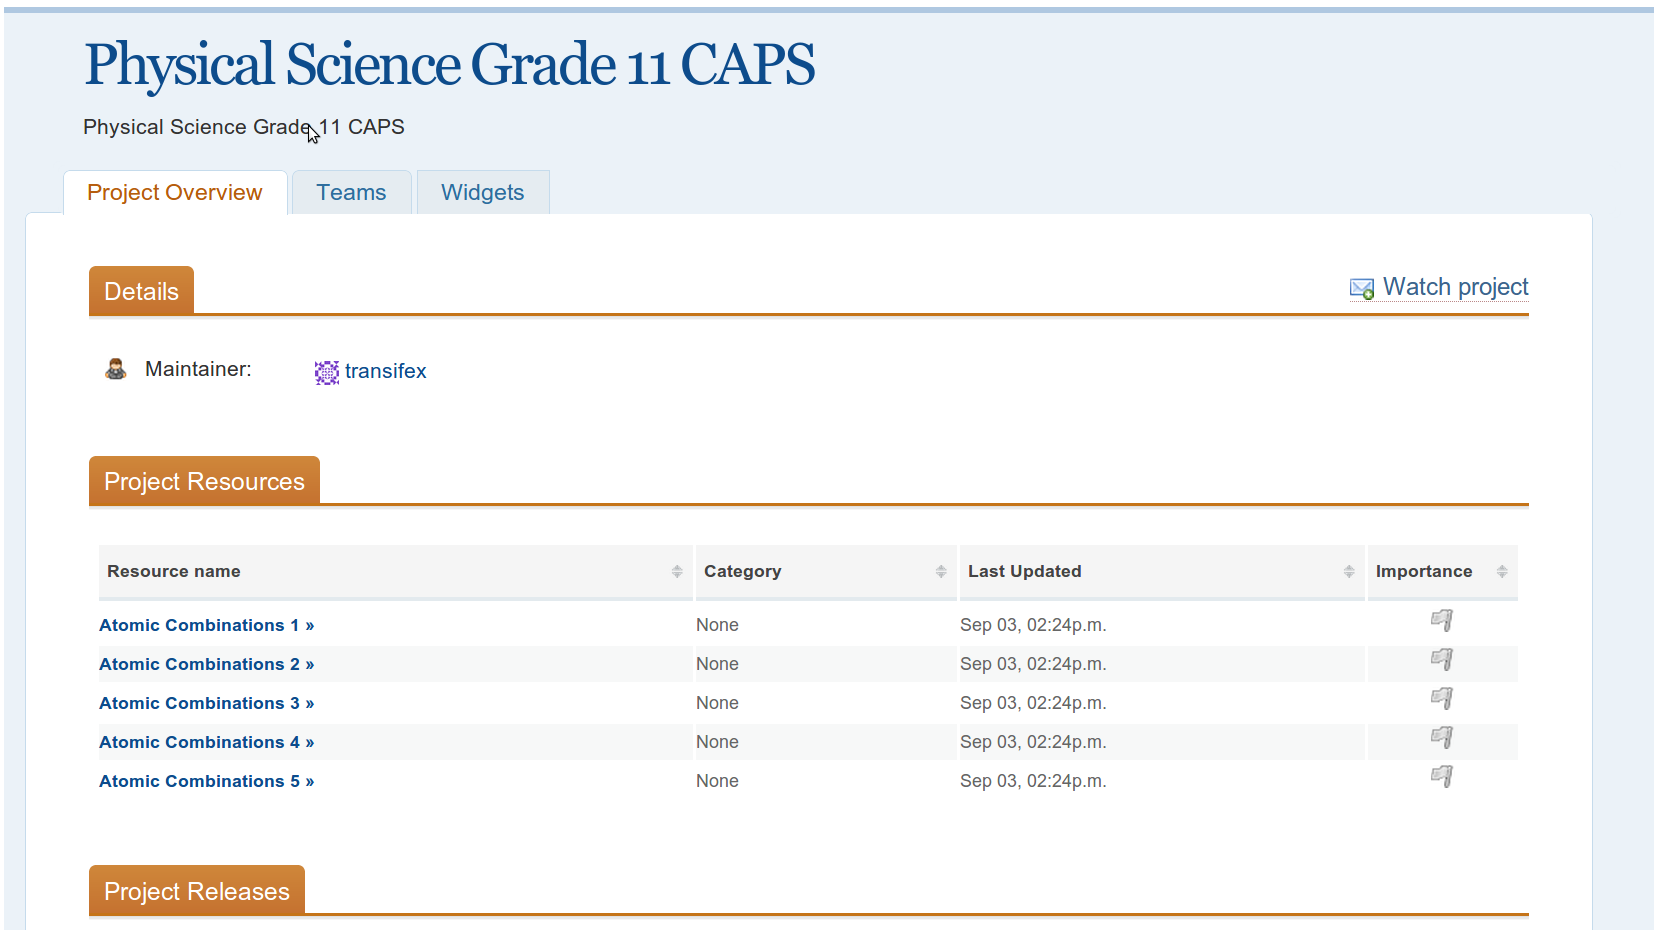
\includegraphics[width=0.8\paperwidth]{images/selectresource.png}}
\end{center}
This will take you to the page detailing the languages for this resource:
\begin{center}
    \centerline{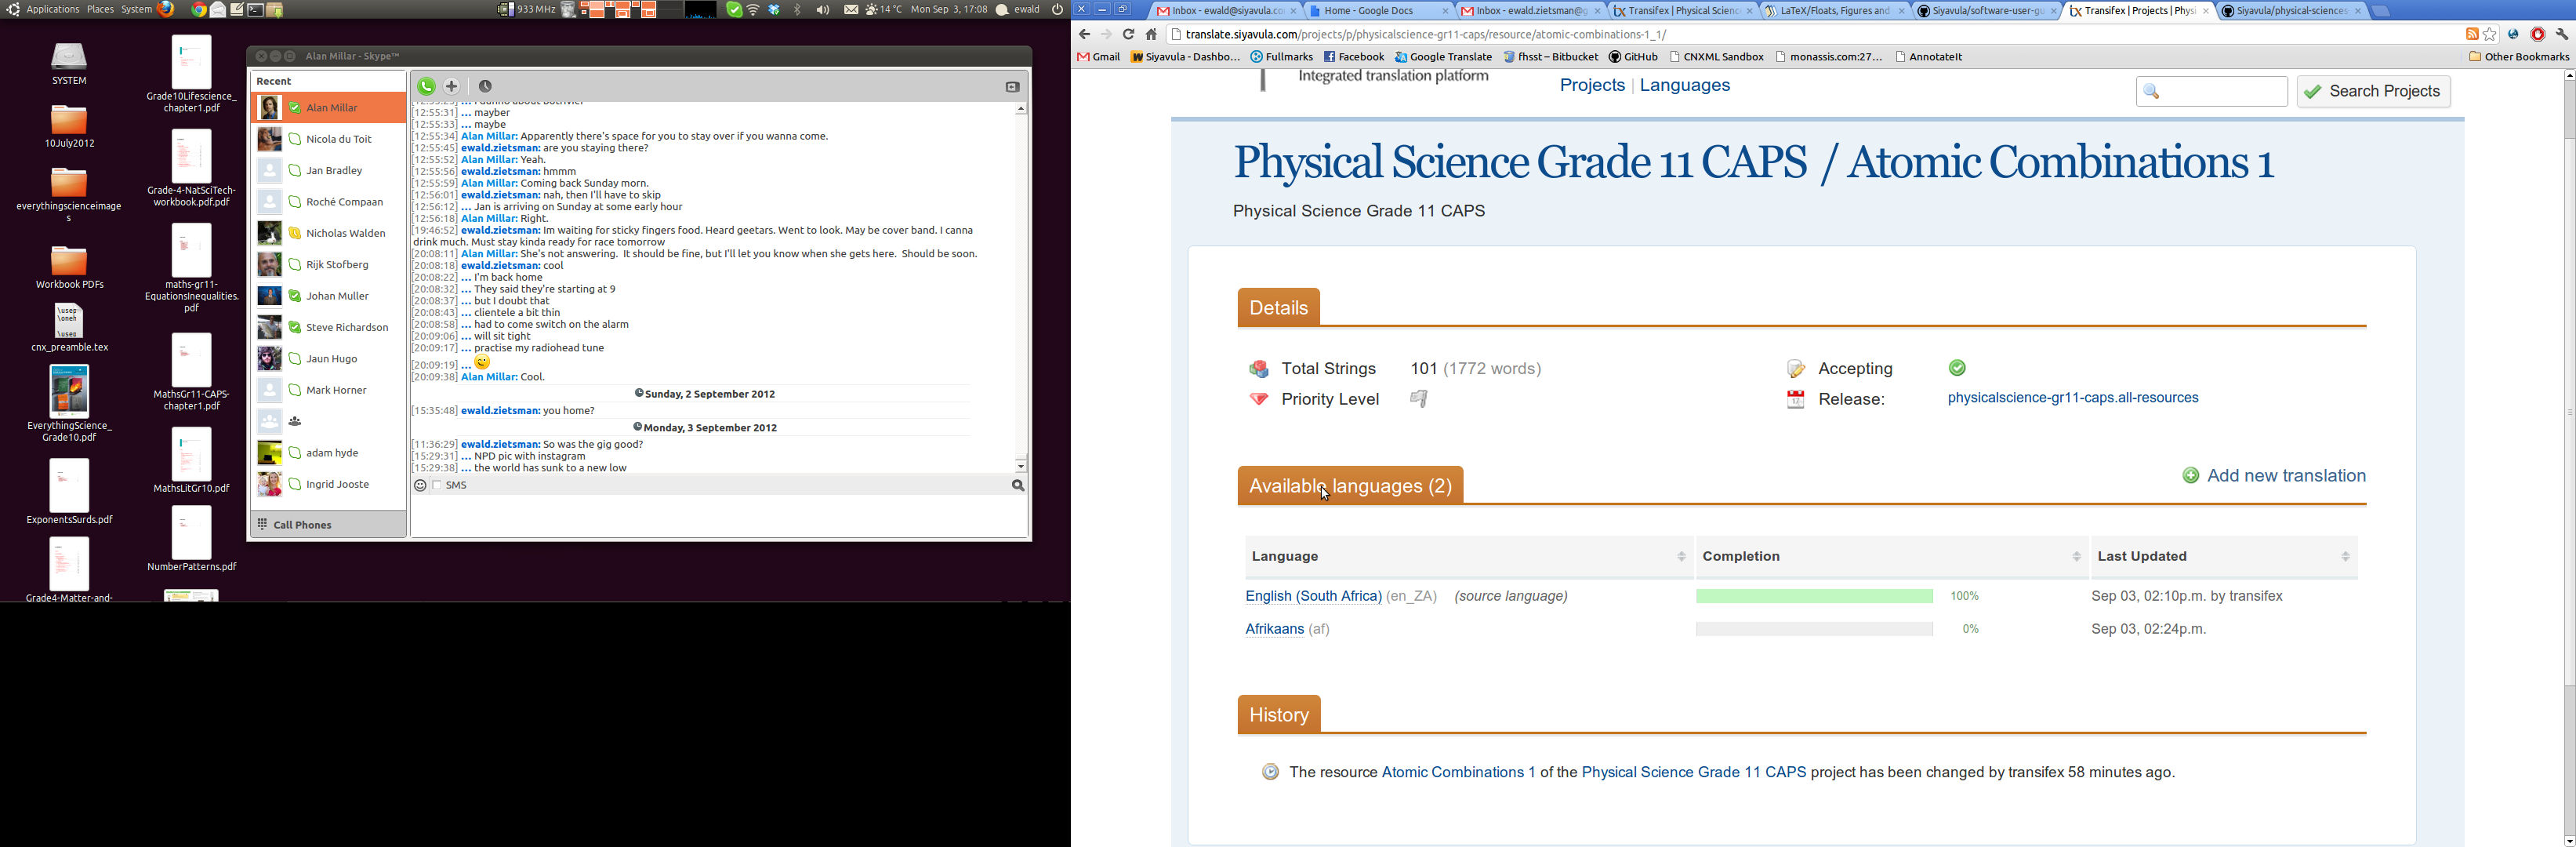
\includegraphics[width=0.8\paperwidth]{images/availablelanguages.png}}
\end{center}

If you are going to translate into Afrikaans, click on the link that says ``Afrikaans''. You will be presented with a pop-up box:
\begin{center}
    \centerline{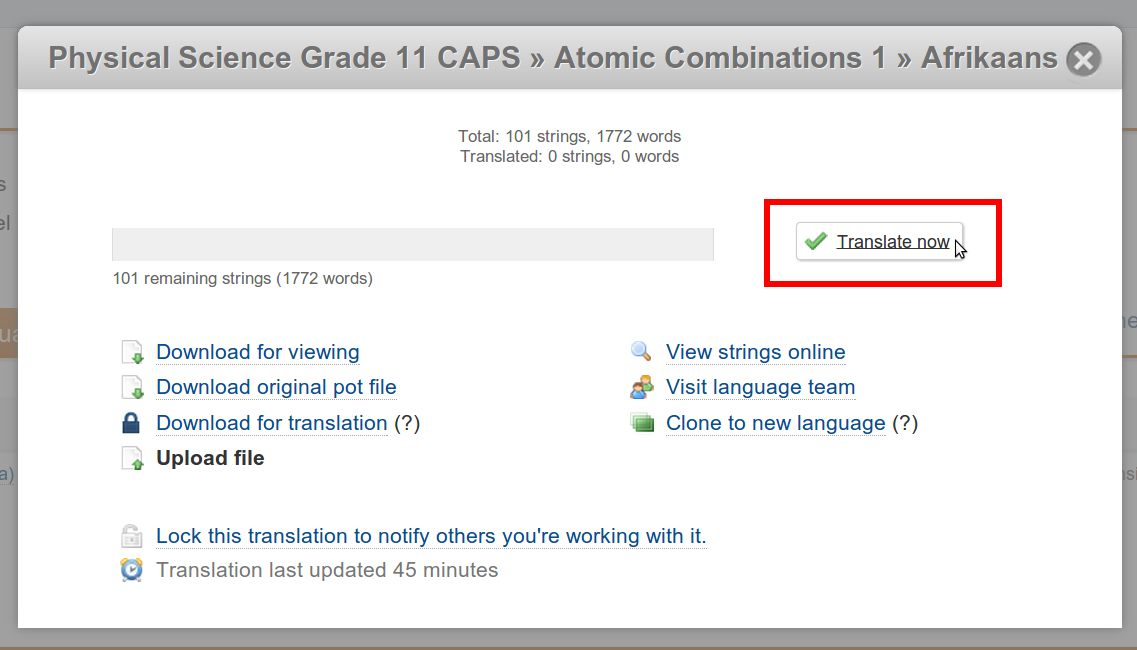
\includegraphics[width=0.8\paperwidth]{images/translatenow.png}}
\end{center}
Click on the button that says ``Translate now''. This will take you to the online translation editor.



\section*{Step 3: Translating strings online}
You should find yourself in the online translation editor. This is where the translations occur. The window on the left shows the source language strings (English in our case) and on the right you may see some Afrikaans strings or empty boxes, where the strings have not been translated yet. It looks like this:
\begin{center}
    \centerline{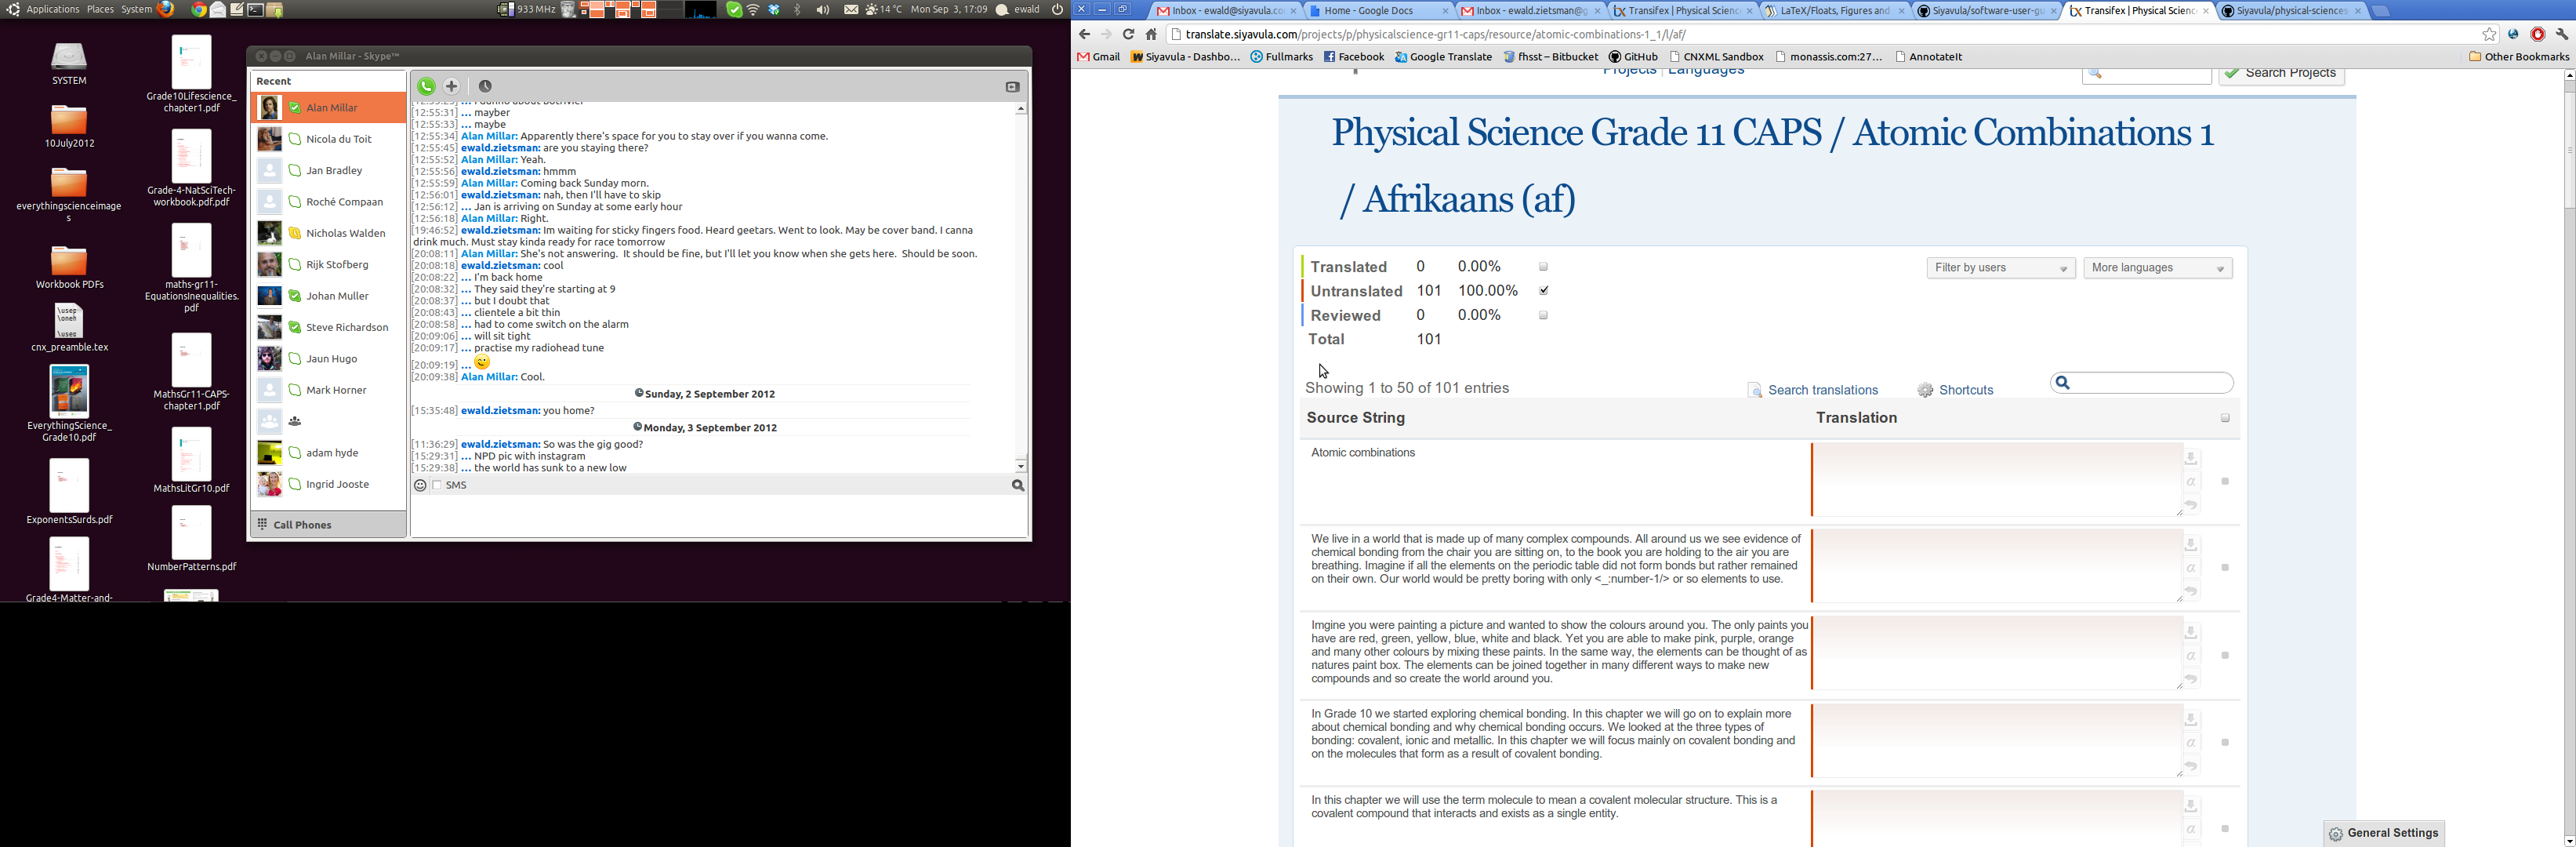
\includegraphics[width=0.8\paperwidth]{images/translatestrings.png}}
\end{center}


To start translating, click on the empty box next to an English string and enter the translation. It may look something like:
\begin{center}
    \centerline{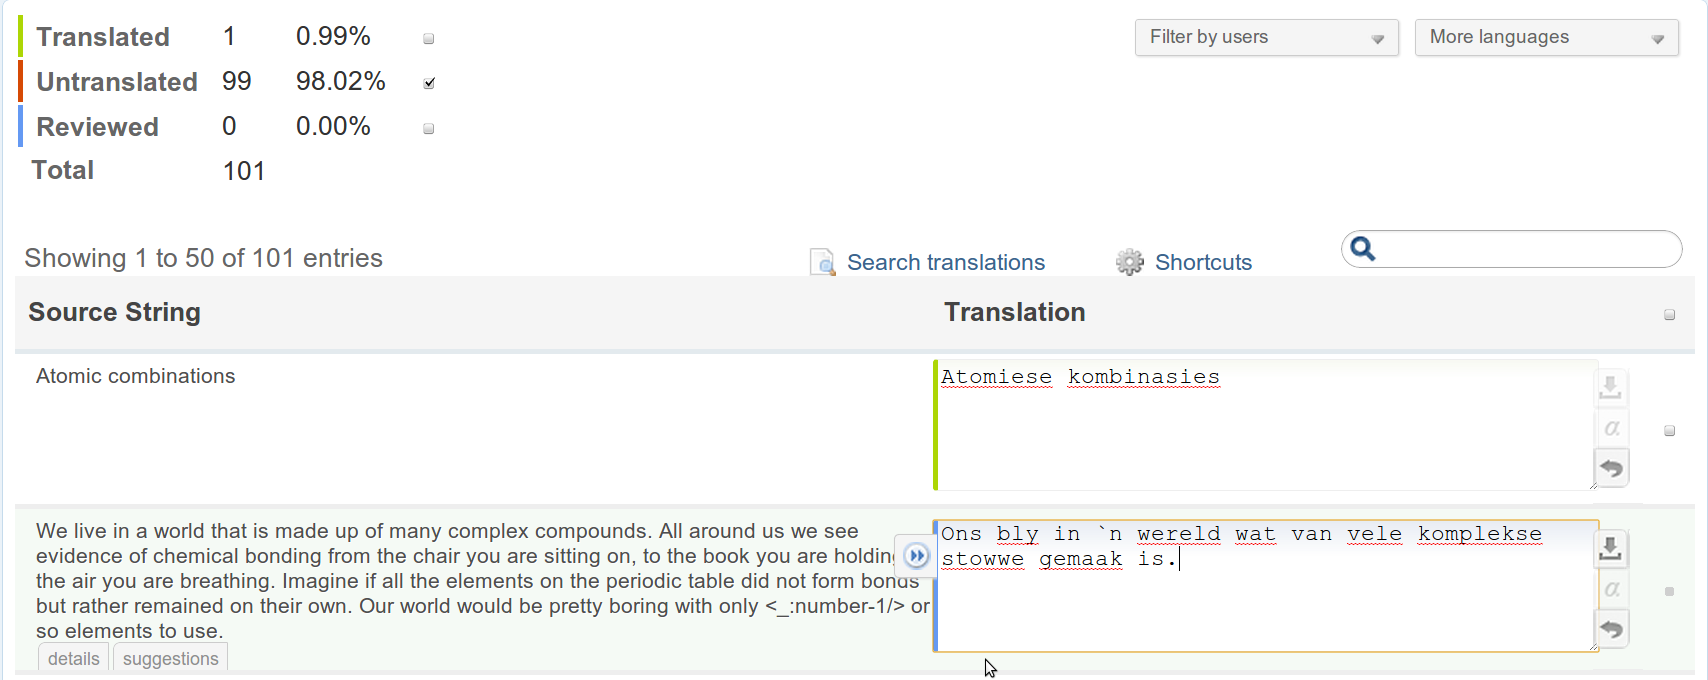
\includegraphics[width=0.8\paperwidth]{images/translating.png}}
\end{center}

When you are done you can hit the save button next to the box:
\begin{center}
    \centerline{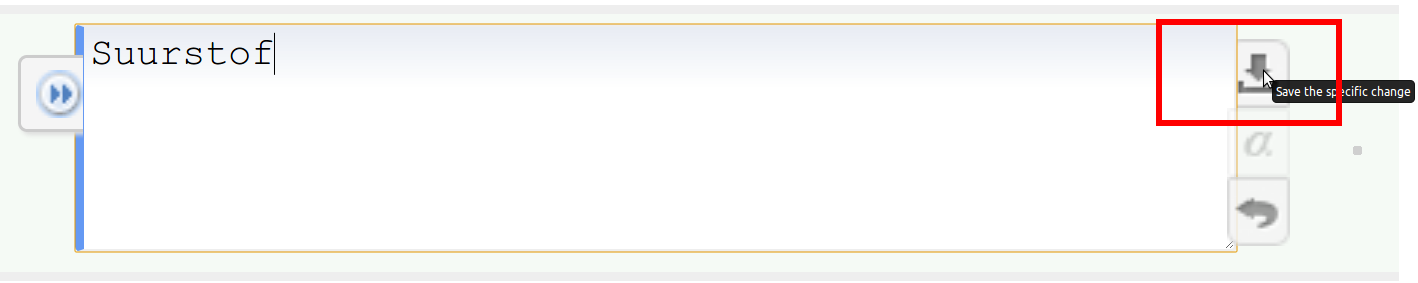
\includegraphics[width=0.8\paperwidth]{images/saving.png}}
\end{center}
You can also just hit the \texttt{Tab} button on your keyboard to save the string and move to the next box automatically. When a string is saved, the left side of the box containing it turns green.


In some cases the translated string is the same as the original string, maybe its a number or a word that is the same in Afrikaans and English. In this case you can hit the \texttt{Copy} button to copy the entire string to the right-hand box. This will save you some time:
\begin{center}
    \centerline{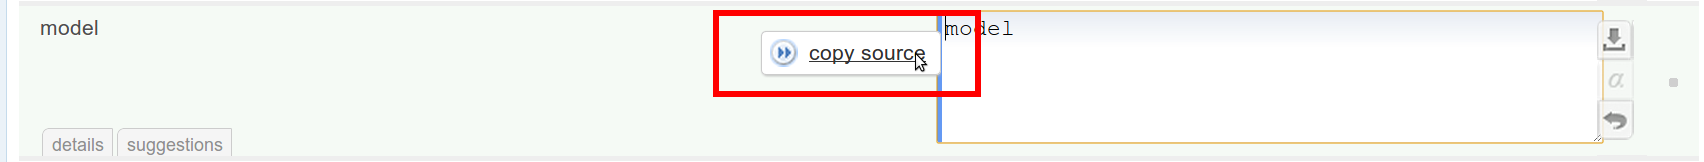
\includegraphics[width=0.8\paperwidth]{images/copy_source.png}}
\end{center}



\textbf{NB!!}

Sometimes you will find English strings that looks like the following:
\begin{verbatim}
Remember that it is only the <_:emphasis-1/> that are involved in bonding, 
and so when diagrams are drawn to show what is happening during bonding, 
it is only these electrons that are shown. Dots or crosses represent electrons 
in different atoms.
\end{verbatim}

The important thing to note is the \verb|<_:emphasis-1/>| that is contained within the string. This is a special marker that Transifex uses to show that a string that will be translated elsewhere is contained within the paragraph or sentence you are currently busy with. The \texttt{emphasis} means the the string is contained within a piece of text marked as \textbf{bold} or \textit{italics} in the book and as such will be translated on its own. \textbf{Please make sure that you include this special marker in your translated string}. If you forget to include it, Transifex will warn you about it. You may see something like:
\begin{center}
    \centerline{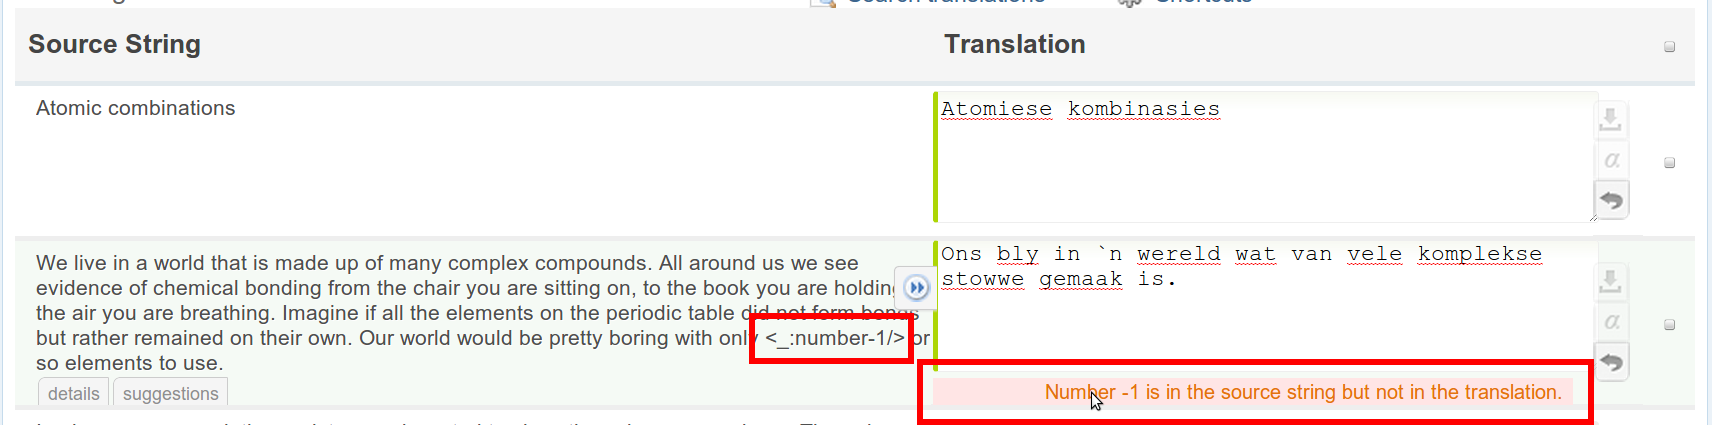
\includegraphics[width=0.8\paperwidth]{images/extra_tags.png}}
\end{center}
The warning will dissappear if you include the entire marker \verb|<_:emphasis-1/>| in the text:
\begin{center}
    \centerline{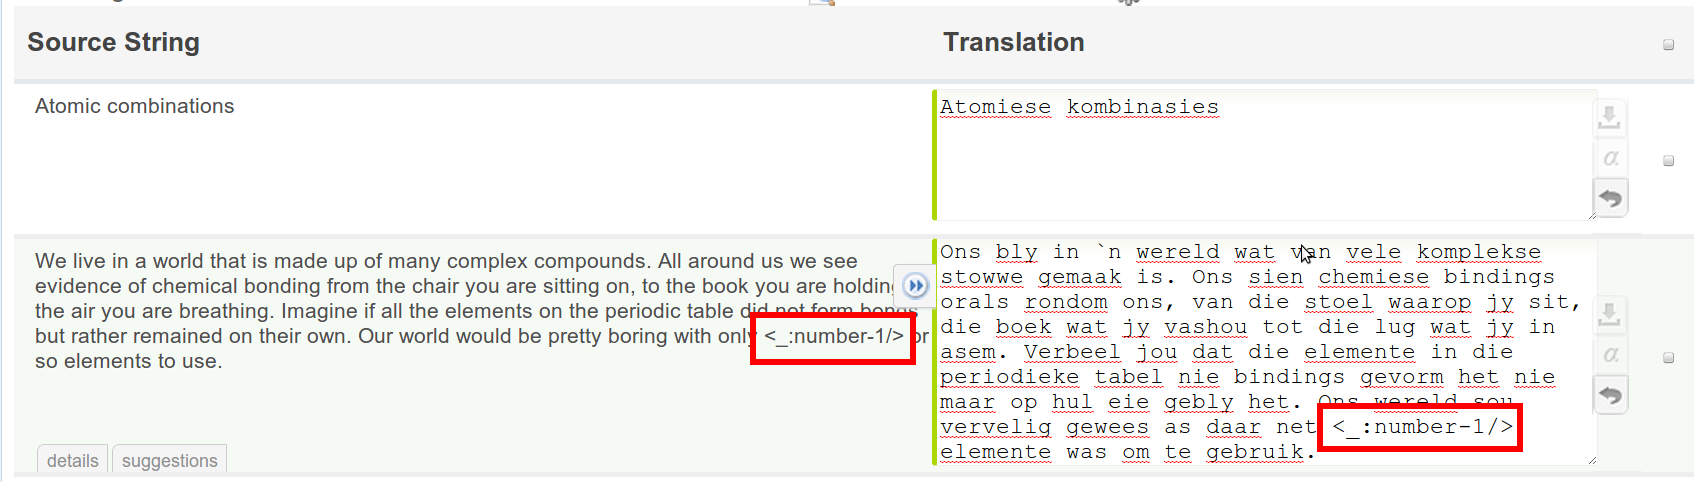
\includegraphics[width=0.8\paperwidth]{images/extra_tags-2.png}}
\end{center}
\textbf{Note:} in the screenshots above the special marker was called \verb|<_:number-1/>|. You will see various kinds of markers starting with \verb|<_:| and ending with \verb|/>| while you do translations. Please remember to include them in the translated strings. Many of them contain special commands that denote chemical symbols, units, numbers etc.

Sometimes it can be difficult to translate a string properly if you cannot see the strings contained within the special markers. In these cases it will help if you consult the PDF version of the chapter you are working on. You should be able to hit \texttt{ctrl} and \texttt{f} simultaneously on your keyboard while inside your PDF reader, that will bring up a search box into which you can type the english string you are translating. This will find that string for you in the document and let you scrutinise the full original string in context.


\section*{Step 4: Reviewing translations}

If you are reviewing other people's translations, you can mark them as reviewed and correct by clicking the checkbox next to the translated string. This checkbox is marked on the image below with the red box on the right. If you have a suggestion for a different or better translation, you can click the \texttt{suggestions} tab beneath the English string and enter your suggestion there:
\begin{center}
    \centerline{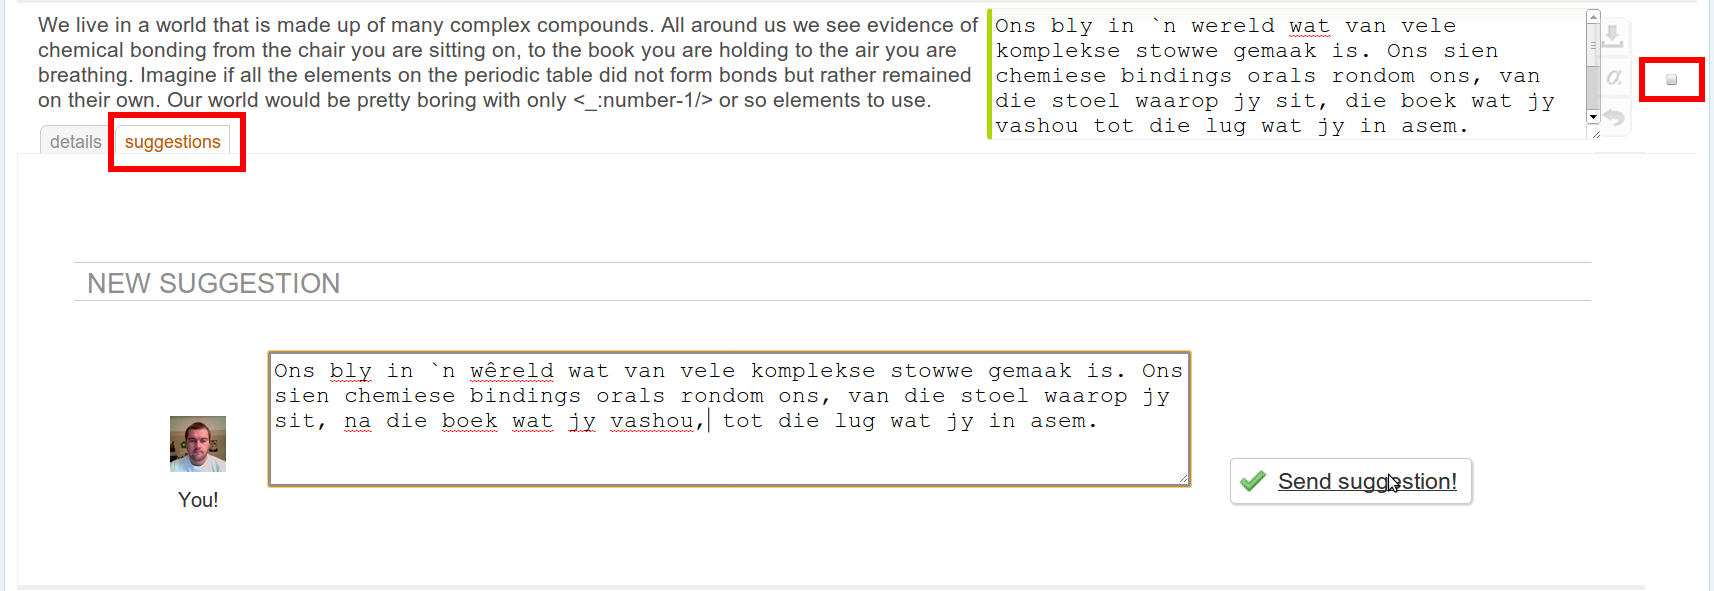
\includegraphics[width=0.8\paperwidth]{images/suggestion.png}}
\end{center}




\section*{Miscellaneous}

\subsection*{Special characters}

To get the \^{e} or \"{e} and other accent signs in Windows: 
\begin{center}
\textbf{Programs » Accessories » System Tools » Character Map}. 
\end{center}
This will open the character map for you. To do the same in Ubuntu Linux use: \textbf{<Alt>-<F2>} and type ``character map''.

\subsection*{Reading the original text in context}

It may be useful to have the PDF of the section you are translating open. This will enable you to search for the strings you are translating and view them in context. To search for a string in Adobe Acrobat Reader hit \textbf{<Ctrl>-<F>} in Acrobat Reader and type the string you want to search for. This is a fast way of locating text in a document.

\end{document}
